% Anhang ist manuell erstellt und verwendet nicht das appendix package
\setcounter{section}{0}
\setcounter{subsection}{0}
\renewcommand*\thesection{\Alph{section}}

\chapter{Anhang}
\section{Struktur und Layout}

\begin{figure}[!ht]
  \centering
  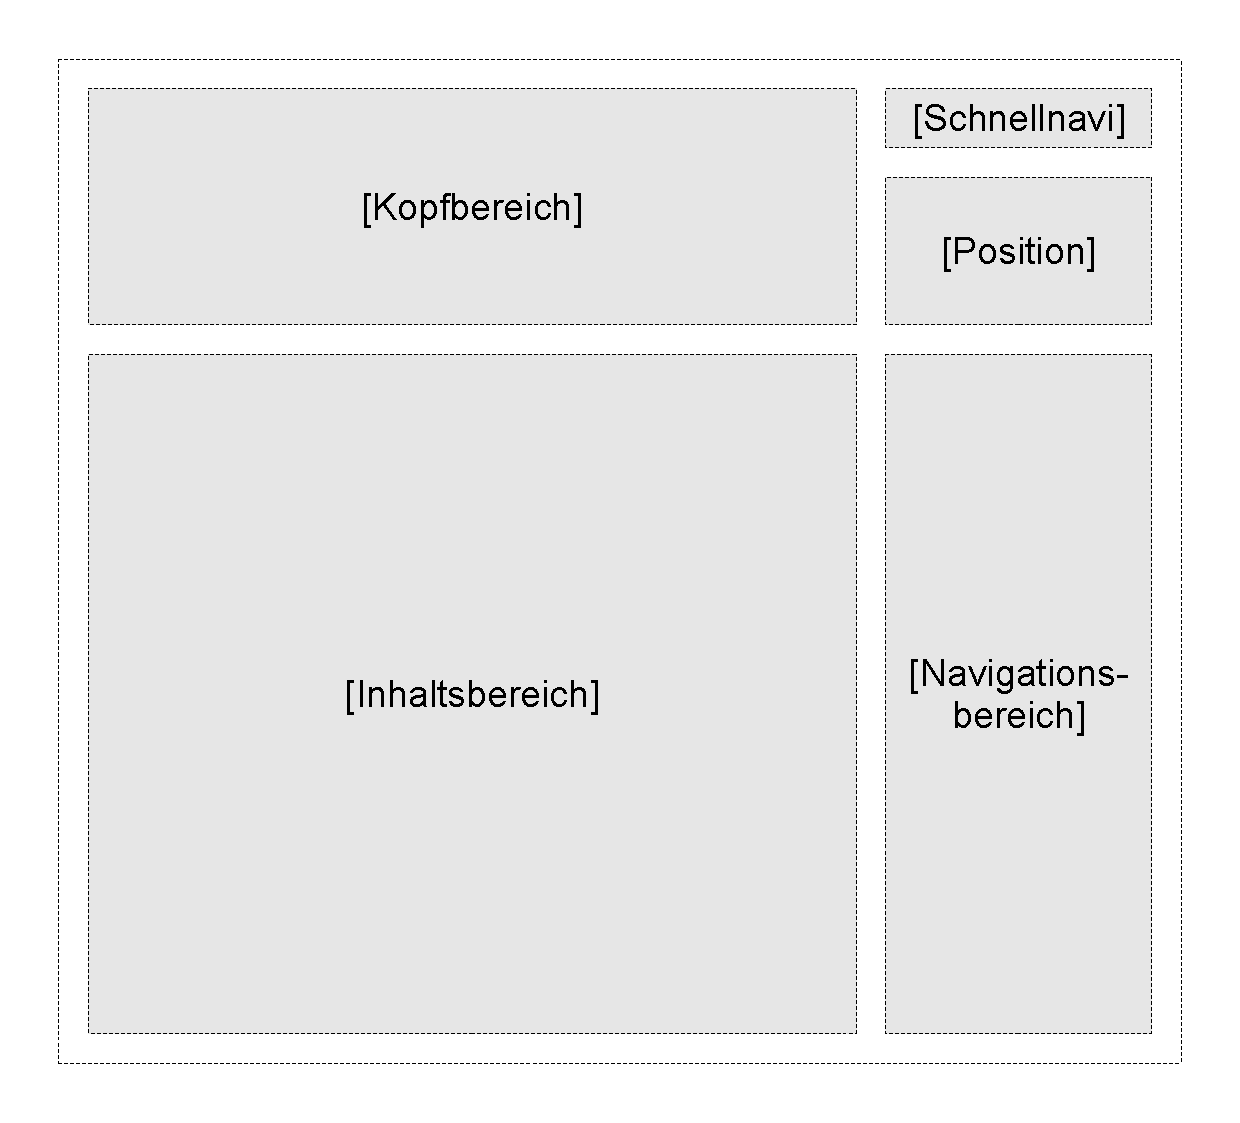
\includegraphics[width=0.6\textwidth]{layout}\\
  \caption{Seitenlayout}
  \label{fig:layout}
\end{figure}

\begin{figure}[!ht]
  \centering
  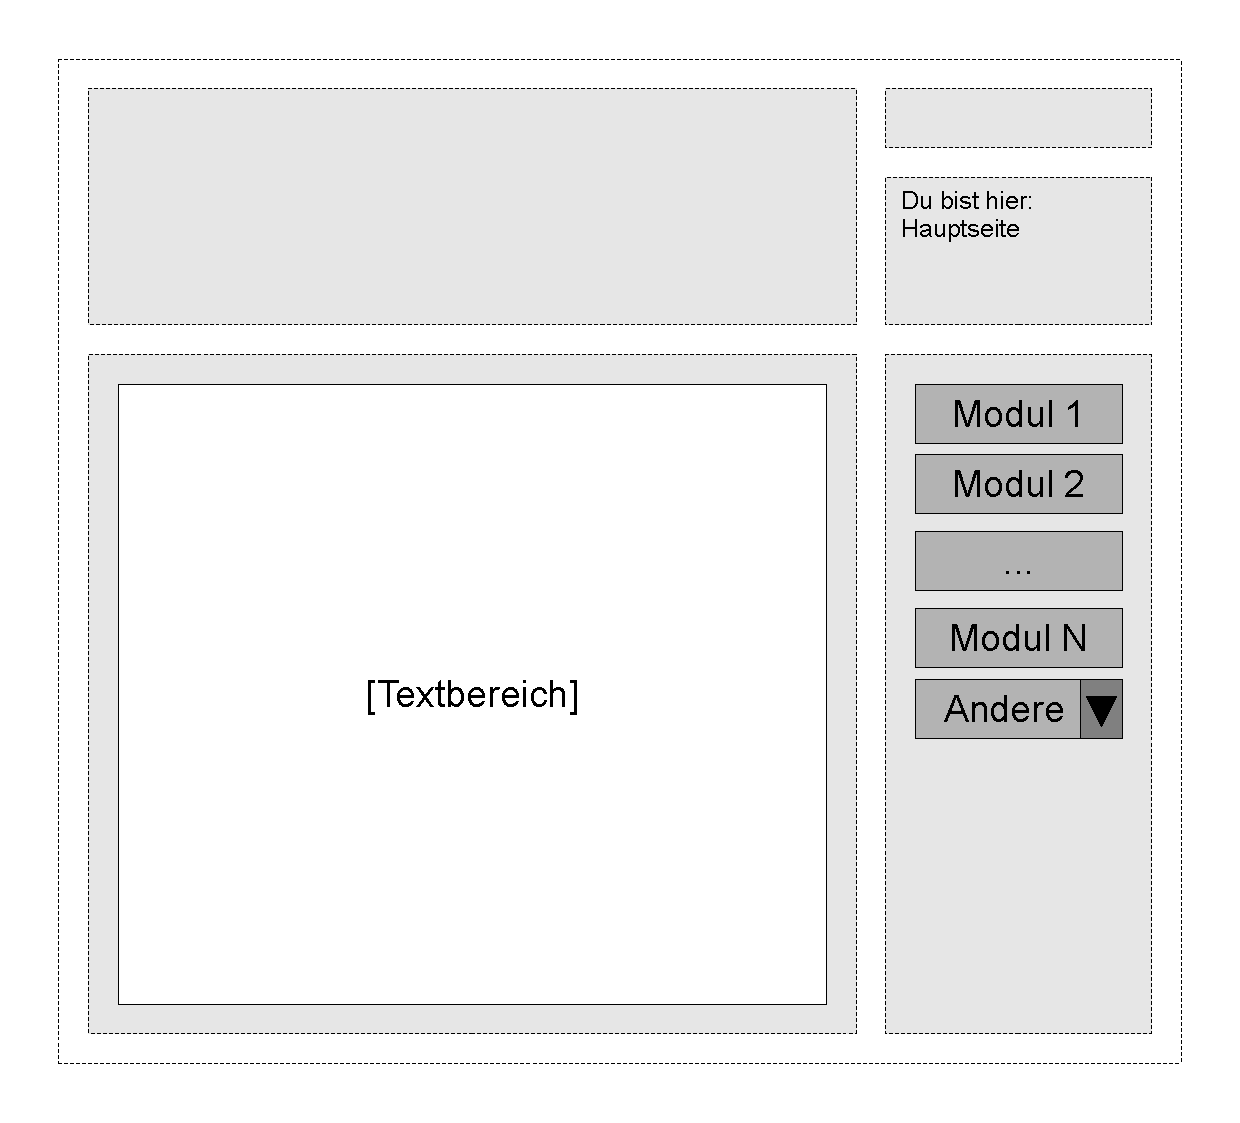
\includegraphics[width=0.6\textwidth]{main-page}\\
  \caption{Hauptseite}
  \label{fig:main-page}
\end{figure}

\begin{figure}[!ht]
  \centering
  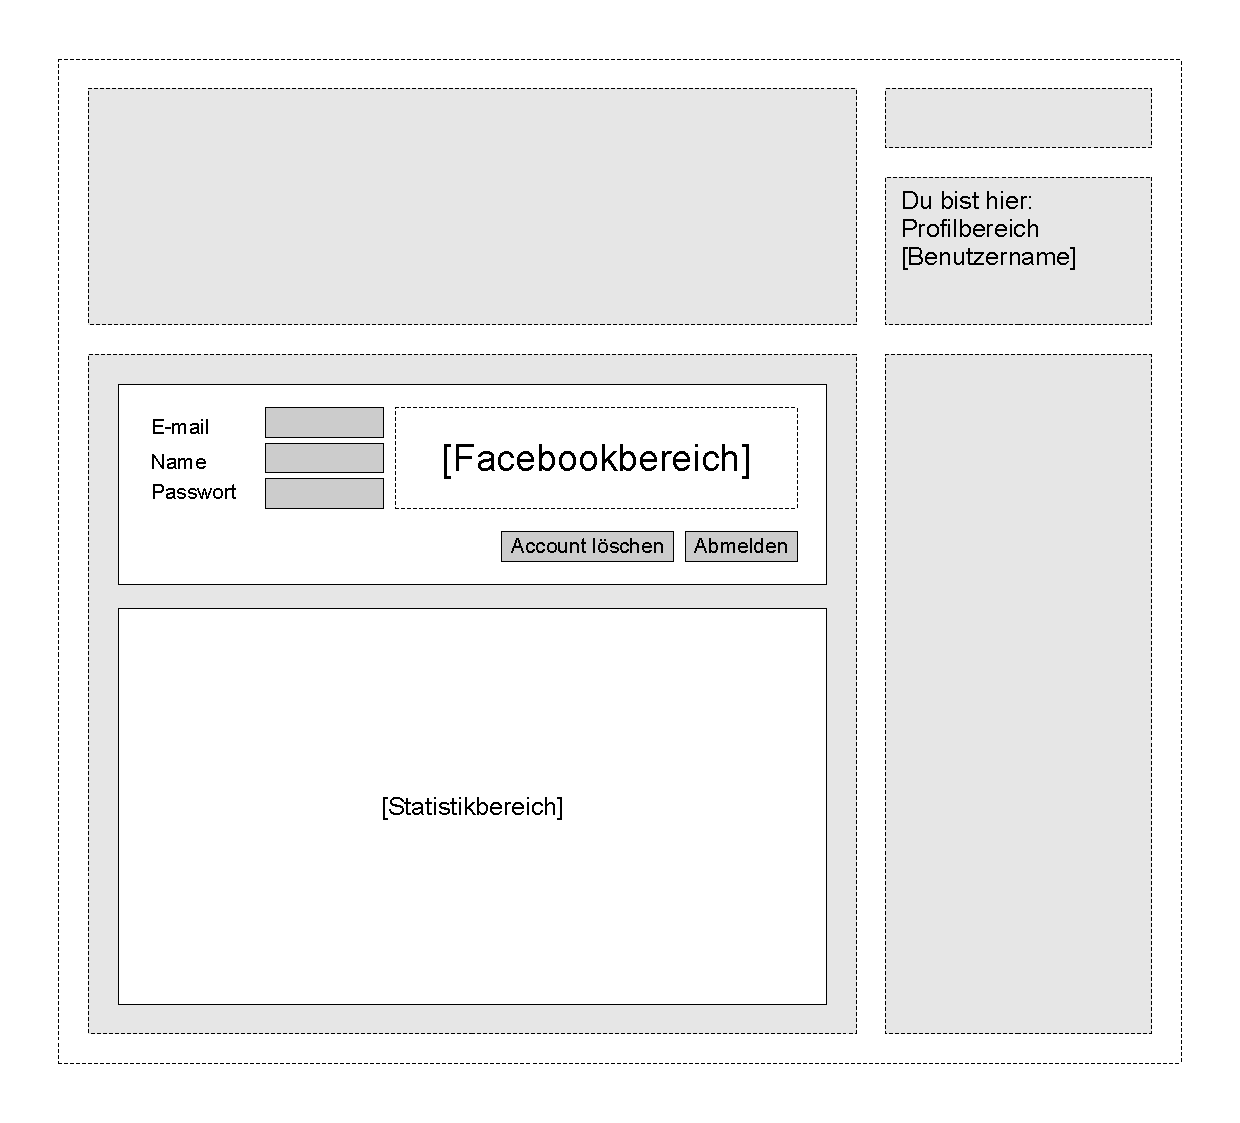
\includegraphics[width=0.6\textwidth]{profile-page}\\
  \caption{Profilseite}
  \label{fig:profile-page}
\end{figure}

\begin{figure}[!ht]
  \centering
  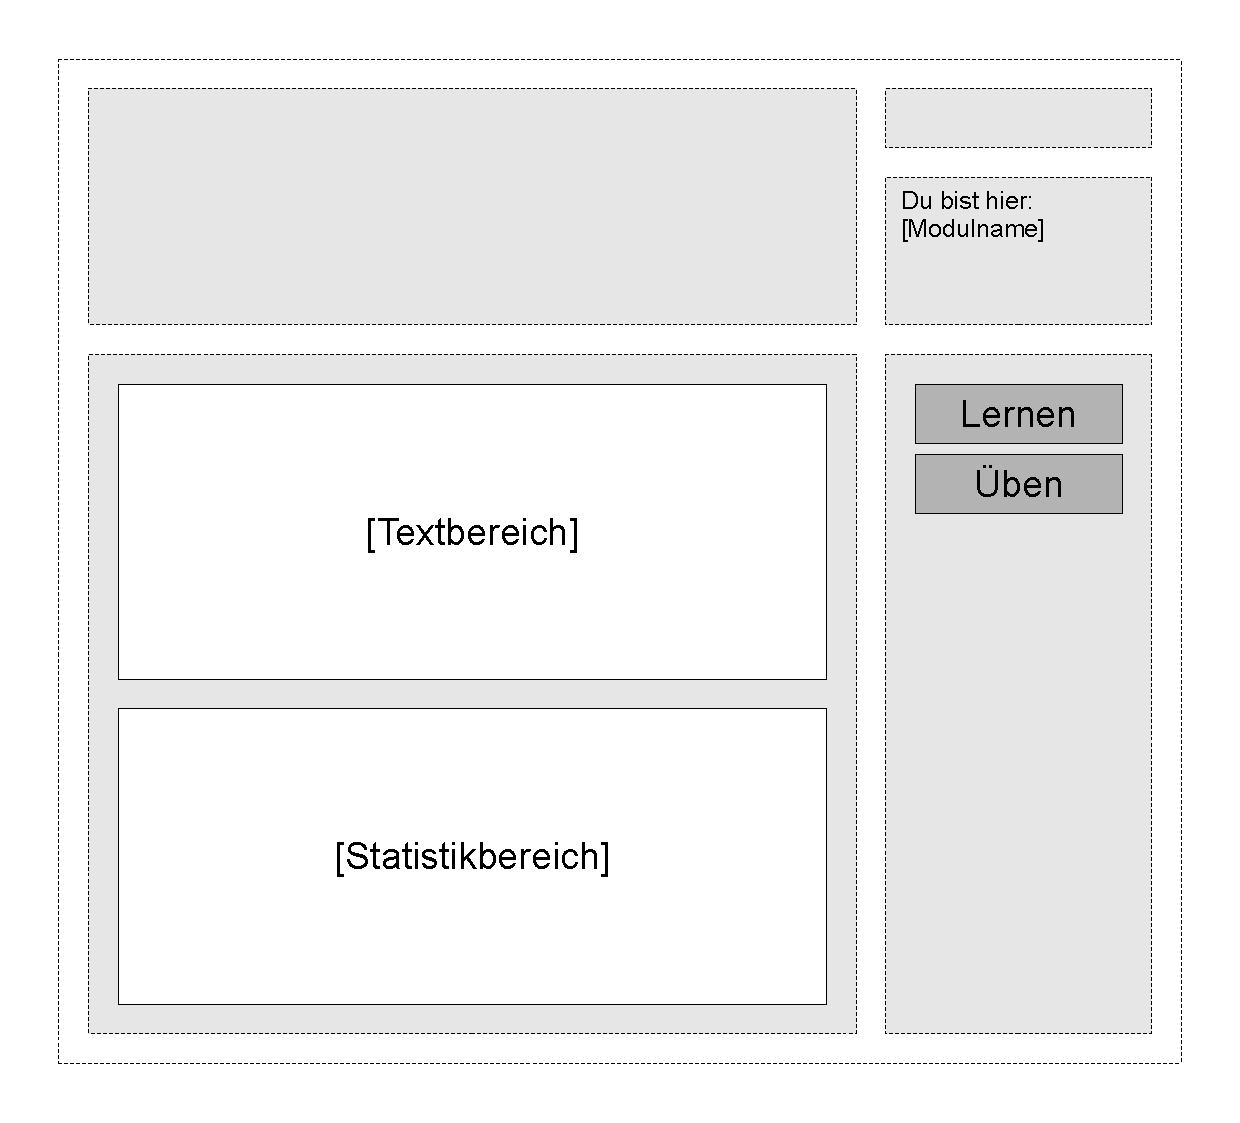
\includegraphics[width=0.6\textwidth]{module-main-page}\\
  \caption{Modulhauptseite}
  \label{fig:module-main-page}
\end{figure}

\begin{figure}[!ht]
  \centering
  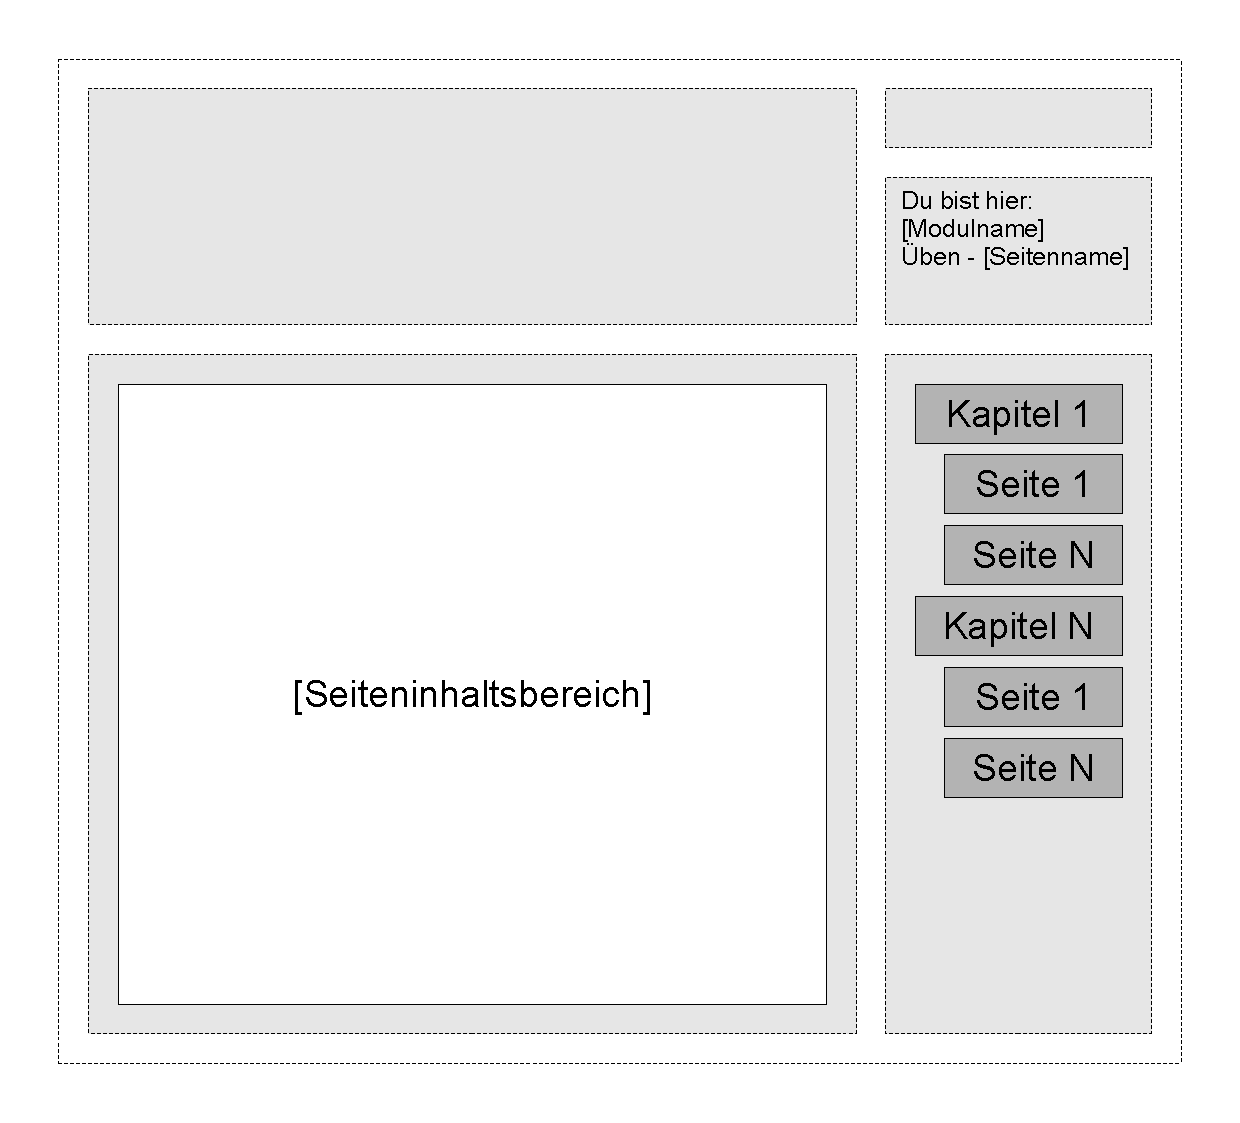
\includegraphics[width=0.6\textwidth]{module-learn-page}\\
  \caption{Modul- Lernseite}
  \label{fig:module-main-page}
\end{figure}

\begin{figure}[!ht]
  \centering
  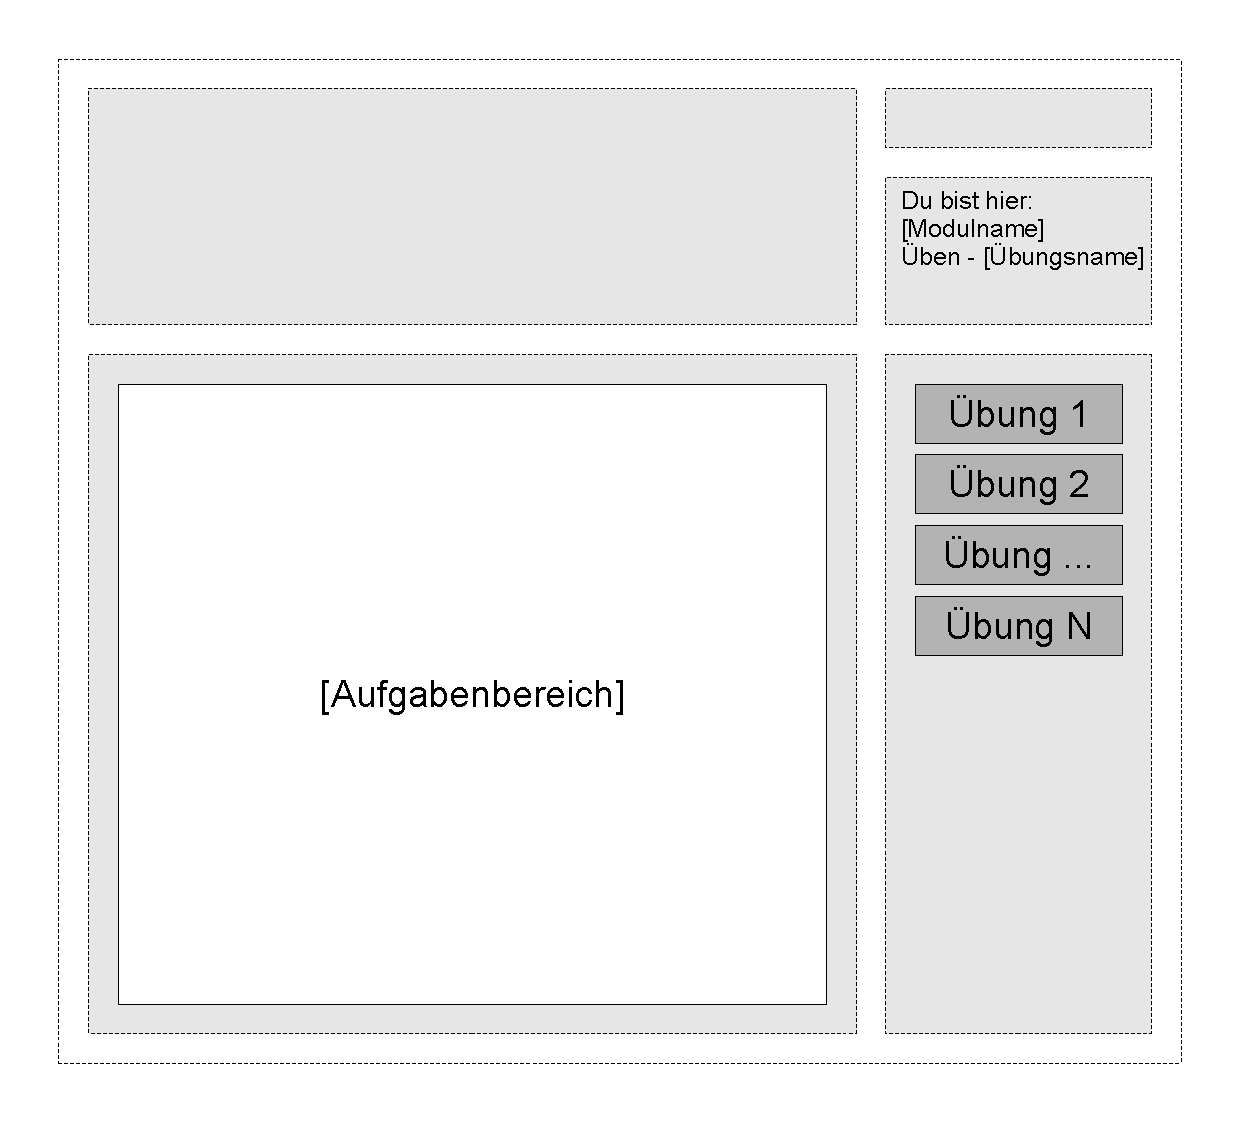
\includegraphics[width=0.6\textwidth]{module-training-page}\\
  \caption{Modul- Übungsseite}
  \label{fig:module-training-page}
\end{figure}

\section{Modul Mathematik}
\subsection{Texte}
\subsection{Icons}
